\documentclass[tikz,border=12pt]{standalone}
% Estilo comum dos esquemas vetoriais das aulas da GA033.
\usepackage[T1]{fontenc}
\usepackage[utf8]{inputenc}
\usepackage{lmodern}
\usepackage{amsmath,amssymb}
\usetikzlibrary{arrows.meta,positioning,calc,fit,matrix,decorations.pathreplacing,backgrounds,shapes.geometric}
\definecolor{lnccblue}{HTML}{075AC0}
\definecolor{ink}{HTML}{242A31}
\definecolor{muted}{HTML}{647080}
\definecolor{lightblue}{HTML}{EFF5FC}
\definecolor{teal}{HTML}{197C83}
\definecolor{orange}{HTML}{BC6A16}
\tikzset{
  every node/.style={font=\sffamily\fontsize{15}{18}\selectfont,text=ink},
  box/.style={draw=lnccblue,line width=0.9pt,fill=lightblue,inner sep=9pt,align=center},
  flow/.style={-{Stealth[length=3mm,width=2mm]},draw=lnccblue,line width=1pt},
  point/.style={circle,draw=lnccblue,fill=white,line width=1.2pt,minimum size=3.2mm,inner sep=0pt},
  label/.style={font=\sffamily\fontsize{13}{16}\selectfont,text=muted},
  heading/.style={font=\sffamily\bfseries\fontsize{16}{19}\selectfont,text=lnccblue}
}
% Impede setas horizontais involuntariamente invertidas após editar os nós.
\newdimen\origemseta
\newdimen\destinoseta
\newcommand{\verificarsetadireita}[2]{%
  \pgfextractx{\origemseta}{\pgfpointanchor{#1}{east}}%
  \pgfextractx{\destinoseta}{\pgfpointanchor{#2}{west}}%
  \advance\origemseta by 4mm%
  \ifdim\destinoseta>\origemseta\else
    \PackageError{diagramas}{Conector sem espaco entre #1 e #2}{Afaste os nos antes de compilar.}%
  \fi
}

\begin{document}
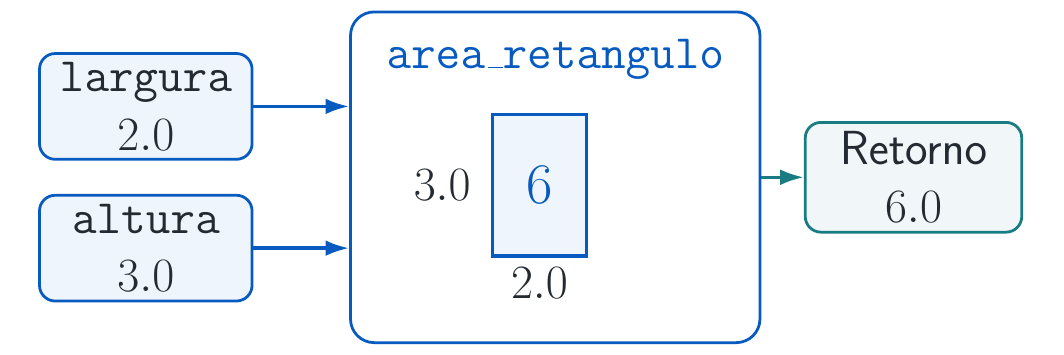
\begin{tikzpicture}[
  x=1cm,y=1cm,every node/.append style={font=\sffamily\fontsize{17}{21}\selectfont},
  entrada/.style={draw=lnccblue,fill=lightblue,rounded corners=2mm,line width=1pt,
    align=center,minimum width=2.7cm,minimum height=1.3cm},
  seta/.style={-{Latex[length=3mm,width=2mm]},draw=lnccblue,line width=1.2pt}
]
\path[use as bounding box] (-.1,-1.9) rectangle (12.7,1.9);
\node[entrada] (largura) at (1.4,.9) {\texttt{largura}\\$2.0$};
\node[entrada] (altura) at (1.4,-.9) {\texttt{altura}\\$3.0$};
\node[draw=lnccblue,fill=white,rounded corners=3mm,line width=1pt,
  minimum width=5.2cm,minimum height=4.2cm] (funcao) at (6.6,0) {};
\node[text=lnccblue,font=\sffamily\fontsize{17}{21}\selectfont\bfseries] at (6.6,1.5) {\texttt{area\_retangulo}};
\draw[draw=lnccblue,fill=lightblue,line width=1.1pt] (5.8,-1.0) rectangle (7.0,.8);
\node[text=ink,font=\sffamily\fontsize{16}{20}\selectfont] at (6.4,-1.35) {$2.0$};
\node[text=ink,font=\sffamily\fontsize{16}{20}\selectfont,anchor=east] at (5.65,-.1) {$3.0$};
\node[text=lnccblue,font=\sffamily\fontsize{22}{26}\selectfont] at (6.4,-.1) {$6$};
\node[entrada,draw=teal,fill=teal!6,minimum width=2.75cm] (retorno) at (11.15,0) {Retorno\\$6.0$};
\verificarsetadireita{largura}{funcao}
\verificarsetadireita{altura}{funcao}
\verificarsetadireita{funcao}{retorno}
\draw[seta] (largura.east) -- (funcao.west |- largura.east);
\draw[seta] (altura.east) -- (funcao.west |- altura.east);
\draw[seta,draw=teal] (funcao.east) -- (retorno.west);
\end{tikzpicture}
\end{document}
